


\newcommand{\drawtruss}[1][1]{%
\begin{center}
\begin{tikzpicture}[scale=#1]
\draw (0,0) -- node[left,magenta]{$1$} (1,1.71) -- node[right,magenta]{$3$} (2,0) -- node[above,magenta]{$2$} cycle;
\draw (2,0) -- node[left,magenta]{$5$} (3,1.71) -- node[above,magenta]{$4$} (1,1.71) -- cycle;
\draw (3,1.71) -- node[right,magenta]{$7$}  (4,0) -- node[above,magenta]{$6$} (2,0) -- cycle;
\draw[blue] (0,0) -- (0.25,-0.425) -- (-0.25,-0.425) -- cycle;
\draw[blue] (4,0) -- (4.25,-0.425) -- (3.75,-0.425) -- cycle;
\draw[thick,red,->] (2,0) --node[right]{10000 N} (2,-0.75);
\end{tikzpicture}
\end{center}
}


\begin{applicationActivities}


\begin{activity}{10}
\begin{itemize}
\item Go to {\tt http://www.cocalc.com} and create an account.
\item Create a project titled ``Linear Algebra Team X'' with your appropriate team number.  Add all team members as collaborators.
\item Open the project and click on ``New''
\item Give it an appropriate name such as ``Class E2 workbook''.  Make a new Jupyter notebook.
\item Click on ``Kernel'' and make sure ``Octave'' is selected.
\item Type {\tt A=[1 3 4 ; 2 5 7]} to store the matrix $\begin{bmatrix} 1 & 3 & 4 \\ 2 & 5 & 7\end{bmatrix}$ in the variable $A$; hold shift when you press enter.
\item Type {\tt rref(A)} to compute the reduced row echelon form of $A$.
\end{itemize}
\end{activity}

\begin{remark}
If you need to find the reduced row echelon form of a matrix during class, you should feel free to use CoCalc/Octave.
\ \\
\ \\
You can change a cell from ``Code'' to ``Markdown'' or ``Raw'' to put comments around your calculations such as Activity numbers.
\end{remark}

\begin{activity}{8}
Consider our system of equations from above.
 \[
		\begin{alignedat}{4}
   		  3x_1 &\,-\,& 2x_2 &\,+\,& 13x_3 &\,=\,& 6 \\
   		  2x_1 &\,-\,& 2x_2 &\,+\,& 10x_3 &\,=\,& 2 \\
   		  -x_1 &\,+\,& 3x_2 &\,-\,&  6x_3 &\,=\,& 11
   		\end{alignedat}
\]

Convert this to an augmented matrix, use CoCalc to compute the reduced row echelon form, and convert back to a simpler system of equations to solve this system.  Write your solution on your whiteboard.
\end{activity}

\begin{activity}{7}
Consider our system of equations from above.
 \[
		\begin{alignedat}{4}
   		  3x_1 &\,-\,& 2x_2 &\,+\,& 13x_3 &\,=\,& 6 \\
   		  2x_1 &\,-\,& 2x_2 &\,+\,& 10x_3 &\,=\,& 2 \\
   		  -x_1 &\,\,&  &\,-\,&  3x_3 &\,=\,&1
   		\end{alignedat}
\]

Convert this to an augmented matrix, use CoCalc to compute the reduced row echelon form, and convert back to a simpler system of equations to solve this system.  Write your solution on your whiteboard.
\end{activity}

\begin{activity}{10}
  Consider the following matrix.
  \[
    A = \begin{bmatrix}[ccc|c]
      1 & 2 & 3 & 1\\
      2 & 4 & 8 & 0
    \end{bmatrix}
  \]
  \begin{subactivity}
    Find \(\RREF(A)\) (Use CoCalc).
  \end{subactivity}
  \begin{subactivity}
    How many solutions does the corresponding linear system have?
  \end{subactivity}
\end{activity}

\begin{activity}{10}
Consider the (simpler) system from the previous problem:
	\begin{alignat*}{3}
		x_1 &+ 2x_2 & &= 4\\
	     	 & &x_3 &= -1
	\end{alignat*}
\begin{subactivity}
Let $x_1=a$ and write the solution set in the form
\( \left\{ \begin{bmatrix} a \\ ? \\ ? \end{bmatrix} \,\middle|\, a \in \IR \right\} \)
\end{subactivity}
\begin{subactivity}
Let $x_2=b$ and write the solution set in the form
\( \left\{ \begin{bmatrix} ? \\ b \\ ? \end{bmatrix} \,\middle|\, b \in \IR \right\} \)
\end{subactivity}
\begin{subactivity}
Which of these was easier?  What features of the RREF matrix \[\begin{bmatrix}[ccc|c] 1 & 2 & 0 & 4 \\ 0 & 0 & 1 & -1 \end{bmatrix}\] cause this?
\end{subactivity}
\end{activity}

\begin{definition}
If a matrix is in reduced row echelon form, a \term{pivot} is an entry satisfying
\begin{enumerate}[1.]
\item It is $1$
\item Everything else in the same row but to the left of it is zero
\item Everything else in the same column is zero.
\end{enumerate}

For example, the pivots are circled in

\[\begin{bmatrix}[ccc|c] \circledNumber{1} & 2 & 0 & 4 \\ 0 & 0 & \circledNumber{1} & -1 \end{bmatrix}\]
\end{definition}


\begin{activity}{5}
Circle the pivots in each matrix below.
\begin{multicols}{2}
\[ \begin{bmatrix}[cccc|c] 1 & 1 & 0 & 0 & 2 \\ 0 & 0 & 1 & 0 &  0 \\ 0 & 0 & 0 &  1 & 1 \end{bmatrix} \]
\[ \begin{bmatrix}[cccc|c] 1 & 1 & 0 & 1 & 0 \\ 0 & 0 & 1 & 1 & 0 \\ 0 & 0 & 0 & 0  & 0 \end{bmatrix} \]
\[ \begin{bmatrix}[ccc|c] 1 & 0 & 1 & 2 \\ 0 & 1 & 0 & 1 \end{bmatrix} \]
\[ \begin{bmatrix}[ccc|c] 1 & 0 & 0 & 2 \\ 0 & 1 & 1 & 0 \\ 0 & 0 & 0 & 0 \end{bmatrix} \]
\end{multicols}
\end{activity}

\begin{definition}
The pivots in a matrix correspond to \term{bound variables} in the system of equations.  The remaining variables are called \term{free variables}.

To efficiently solve a system in RREF form, assign letters to free variables and solve for the bound variables.
\end{definition}

\begin{activity}{10}
Find the solution set for the system
\begin{alignat*}{6}
2x_1&\,-\,&2x_2&\,-\,&6x_3&\,+\,&x_4&\,-\,&x_5&\,=\,&3 \\
-x_1&\,+\,&x_2&\,+\,&3x_3&\,-\,&x_4&\,+\,&2x_5 &\,=\,& -3 \\
x_1&\,-\,&2x_2&\,-\,&x_3&\,+\,&x_4&\,+\,&x_5 &\,=\,& 2
\end{alignat*}
by assigning letters to the free variables and solving for the bounded variables.
\end{activity}

\begin{observation}
The solution set to the system
\begin{alignat*}{6}
2x_1&\,-\,&2x_2&\,-\,&6x_3&\,+\,&x_4&\,-\,&x_5&\,=\,&3 \\
-x_1&\,+\,&x_2&\,+\,&3x_3&\,-\,&x_4&\,+\,&2x_5 &\,=\,& -3 \\
x_1&\,-\,&2x_2&\,-\,&x_3&\,+\,&x_4&\,+\,&x_5 &\,=\,& 2
\end{alignat*}
is \[\left\{ \begin{bmatrix} 1+5a+2b \\ 1+2a+3b \\ a \\3+3b \\ b \end{bmatrix}\,\middle|\, a,b\in \IR\right\}.\]
\end{observation}

\begin{observation}
Consider the truss pictured below with two fixed anchor points and a 10000 N load (assume all triangles are equilateral).
\drawtruss

The horizontal and vertical forces must balance at each of the five intersecting nodes.  For example, at the bottom left node
\begin{multicols}{4}
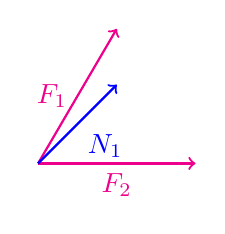
\begin{tikzpicture}
\draw [thick, magenta,->] (0,0) -- node[left]{$F_1$} (1,1.71);
\draw [thick, magenta,->] (0,0) -- node[below]{$F_2$} (2,0);
\draw [thick, blue,->] (0,0) -- node[below right]{$N_1$} (1,1);
\end{tikzpicture}

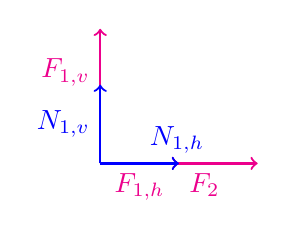
\begin{tikzpicture}
\draw [thick, magenta,->] (0,0) -- node[above left]{$F_{1,v}$} (0,1.71);
\draw [thick, magenta,->] (0,0) -- node[below]{$F_{1,h}$} (1,0);
\draw [thick, magenta,->] (0,0) -- node[below right]{$F_2$} (2,0);
\draw [thick, blue,->] (0,0) -- node[left]{$N_{1,v}$} (0,1);
\draw [thick, blue,->] (0,0) -- node[above right]{$N_{1,h}$} (1,0);
\end{tikzpicture}

Apply basic trig:
\begin{align*}
F_{1,v}&=F_1 \sin(60^\circ) \\ F_{1,h}&=F_1\cos(60^\circ)
\end{align*}

thus
\begin{align*}
F_1 \sin(60^\circ)+N_{1,v} &= 0 \\
F_1 \cos(60^\circ)+N_{1,h}+F_2 &= 0
\end{align*}
\end{multicols}

We adhere to the convention that a compression force on a strut is positive, while a negative force represents tension.
\end{observation}

\begin{activity}{10}
Consider the truss pictured below with two fixed anchor points and a 10000 N load (assume all triangles are equilateral).
\drawtruss

From the bottom left node we obtained 2 equations in the four variables
\begin{itemize}
\item $F_{1}$ (compression force on strut one)
\item $N_{1,v}$ and $N_{1,h}$ (horizontal and vertical components of the normal force from the left anchor)
\item $F_2$ (compression force on strut 2).
\end{itemize}

\begin{subactivity}
Determine how many total equations there will be after accounting for all of the nodes, and and list all of the variables.  You do not need to actually determine all of the equations.
\end{subactivity}
\end{activity}


\begin{activity}{10}
\drawtruss[0.8]
The resulting system is
\begin{alignat*}{12}
N_{1,v} &\,\,& &\,\,& &\,\,& &\,+\,& (\sin(60^\circ))F_1 &\,\,& &\,\,& &\,\,& &\,\,& &\,\,& &\,\,& &\,=\,& 0 \\
        &\,\,& N_{1,h} &\,\,& &\,\,& &\,+\,& (\cos(60^\circ))F_1 &\,+\,&F_2 &\,\,& &\,\,& &\,\,& &\,\,& &\,\,& &\,=\,& 0 \\
        &\,\,&         &\,\,& &\,\,& &\,-\,& (\sin(60^\circ))F_1 &\,\,& &\,-\,&(\sin(60^\circ)F_3 &\,\,& &\,\,& &\,\,& &\,\,& &\,=\,& 0 \\
        &\,\,&         &\,\,& &\,\,& &\,-\,& (\cos(60^\circ))F_1 &\,\,& &\,+\,&(\cos(60^\circ)F_3 &\,+\,&F_4 &\,\,& &\,\,& &\,\,& &\,=\,& 0 \\
        &\,\,&         &\,\,& &\,\,& &\,\,&                     &\,\,& &\,\,&(\sin(60^\circ)F_3 &\,\,& &\,+\,& (\sin(60^\circ))F_5&\,\,& &\,\,& &\,=\,& 10000 \\
        &\,\,&         &\,\,& &\,\,& &\,\,&                     &\,-\,& F_2&\,-\,&(\cos(60^\circ)F_3 &\,\,& &\,+\,& (\cos(60^\circ))F_5&\,+\,&F_6 &\,\,& &\,=\,& 0 \\
        &\,\,&         &\,\,& &\,\,& &\,\,&                     &\,\,& &\,\,&                   &\,\,& &\,-\,& (\sin(60^\circ))F_5&\,\,& &\,-\,& (\sin(60^\circ))F_7&\,=\,& 0 \\
        &\,\,&         &\,\,& &\,\,& &\,\,&                     &\,\,& &\,\,&                   &\,-\,&F_4 &\,-\,& (\cos(60^\circ))F_5&\,\,& &\,+\,& (\cos(60^\circ))F_7&\,=\,& 0 \\
        &\,\,&         &\,\,& N_{2,v} &\,\,& &\,\,&                     &\,\,& &\,\,&                   &\,\,& &\,\,&                    &\,\,& &\,+\,& (\sin(60^\circ))F_7&\,=\,& 0 \\
        &\,\,&         &\,\,& &\,\,&N_{2,h} &\,\,&                     &\,\,& &\,\,&                   &\,\,&    &\,\,&                    &\,-\,& F_6 &\,-\,& (\cos(60^\circ))F_7&\,=\,& 0
\end{alignat*}
Solve this system to determine which struts are compressed and which are in tension.
\end{activity}

\begin{observation}
The determined part of the solution is
\begin{align*}
N_{1,v}=N_{2,v}&=5000 \\
F_1=F_4=F_7&=-5882.4 \\
F_3=F_5=5882.4
\end{align*}

So struts 1,4,7 are in tension, while struts 3 and 5 are compressed.

The forces on struts 2 and 6 (and the horizontal normal forces) are not strictly determined in this setting.
\end{observation}

\end{applicationActivities}
